\chapter{Framework Design}

Our work towards adding more automation to theory development envisions users and library developers writing expressions like 
\begin{lstlisting}
Mononid = combine Unital and Semigroup over Magma
            generate homomorphism, OpenTerms, Simplifier
            using (waist=1,eq=Agda.Builtin.Equality)
\end{lstlisting}
The systems would then provide the theory presentation for \lstmath{Monoid} as a descendant of \lstmath{Unital} and \lstmath{Semigroup}\footnote{The \lstmath{combine} operation is explained in detail in Section~\ref{subsec:combine}} and
the constructions specified in the \lstmath{generate} clause, employing the design decisions in the \lstmath{using} clause.  

The interpreter of the DSL does the transformation from declarative expressions to definitions acceptable by a host language. We suggest an interpreter that consists of three phases as shown in Figure~\ref{fig:staged-interpreter}. 
\begin{figure}
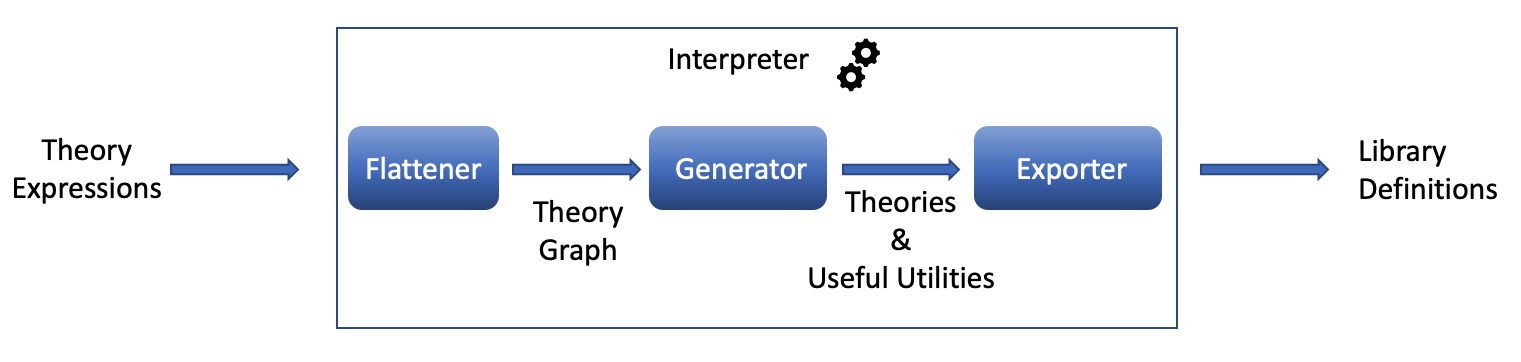
\includegraphics[scale=0.5,width=\linewidth]{figures/interpreter_detailed}
\caption{A $3$-staged interpreter for generating libraries}
\label{fig:staged-interpreter}
\end{figure}

\paragraph{Flattener.} The first stage of the interpreter builds a theory graph of algebraic structures. To provide more conciseness and better reuse, we use combinators to define new theories. The flattener uses expressions built using the combinators to build a theory graph. The problem here is to choose combinators that leverages the mathematical structure by providing expressive morphisms capable of describing the relationship between theories. We discuss our choice of combinators in Chapter~\ref{ch:library}. A strong requirement that we have regarding combinators is to allow computing flattened theories. While it is useful for the system to know that a \lstmath{Group} is a \lstmath{Monoid} with inverse and automate the transportation of theorems proved in \lstmath{Monoid} theory to be used in \lstmath{Group} theory, some potential users might want to use \lstmath{Group}s without caring about how they are built. We want to use combinators that allows both views for users, by avoiding qualified names and dropping and freeness combinators.\ednote{probably need references here.}
%without imposing one of Our library need to support both definitions, by enabling the users to work with flat version of the library. Some operations on theories make this hard to achieve, like dropping and freeness combinators by CASL\ednote{look for a source explaining why they are problematic}. 

\paragraph{Generator.} The input to the generator is a flat theory presentation, the output of the flattener. The generator manipulates the components of a theory presentation generating related constructions based on how they are defined in universal algebra. Therefore, the input theory needs to fit in the universal algebra abstraction of a theory, being a first-order equational theory. Despite this limitation, the algebraic hierarchy until at least \lstmath{Ring}\ednote{or maybe more?} fits in this criteria. We discuss our implementation of the generator in Chapter~\ref{ch:generation}. 

\paragraph{Exporter.} The Flattener and Generator deal with \emph{raw} mathematical definition, keeping system-specific design decision to a minimal. The exporter puts back these decisions. This way we provide customized definitions which increases their usability across different systems, users, and projects. \ednote{add reference to the chapter}. 


